\documentclass{standalone}
\usepackage{tikz}
\usetikzlibrary{patterns, positioning}


\begin{document}
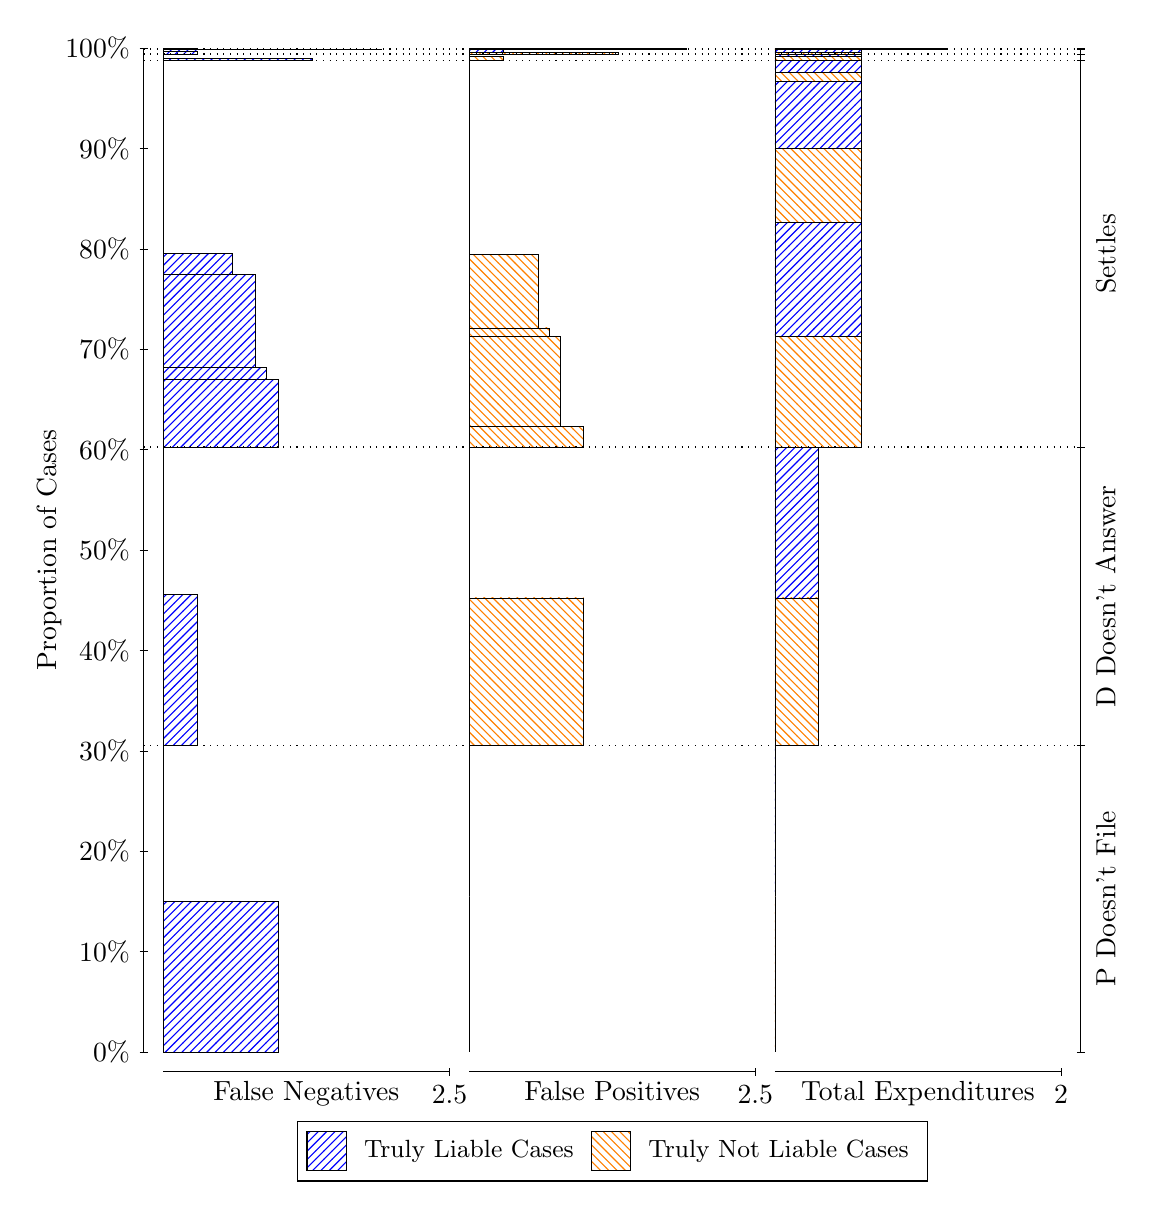
\begin{tikzpicture}
\draw[black, very thin] (1.5,1.75) -- (1.5,14.5);
\node[rotate=90, text=black, anchor=center] at (0.3, 8.125) {Proportion of Cases};
\draw[black, very thin] (1.45,1.75) -- (1.55,1.75);
\node[text=black, anchor=east] at (1.45, 1.75) {0\%};
\draw[black, very thin] (1.45,3.025) -- (1.55,3.025);
\node[text=black, anchor=east] at (1.45, 3.025) {10\%};
\draw[black, very thin] (1.45,4.3) -- (1.55,4.3);
\node[text=black, anchor=east] at (1.45, 4.3) {20\%};
\draw[black, very thin] (1.45,5.575) -- (1.55,5.575);
\node[text=black, anchor=east] at (1.45, 5.575) {30\%};
\draw[black, very thin] (1.45,6.85) -- (1.55,6.85);
\node[text=black, anchor=east] at (1.45, 6.85) {40\%};
\draw[black, very thin] (1.45,8.125) -- (1.55,8.125);
\node[text=black, anchor=east] at (1.45, 8.125) {50\%};
\draw[black, very thin] (1.45,9.4) -- (1.55,9.4);
\node[text=black, anchor=east] at (1.45, 9.4) {60\%};
\draw[black, very thin] (1.45,10.675) -- (1.55,10.675);
\node[text=black, anchor=east] at (1.45, 10.675) {70\%};
\draw[black, very thin] (1.45,11.95) -- (1.55,11.95);
\node[text=black, anchor=east] at (1.45, 11.95) {80\%};
\draw[black, very thin] (1.45,13.225) -- (1.55,13.225);
\node[text=black, anchor=east] at (1.45, 13.225) {90\%};
\draw[black, very thin] (1.45,14.5) -- (1.55,14.5);
\node[text=black, anchor=east] at (1.45, 14.5) {100\%};

\draw[black, very thin] (13.4,1.75) -- (13.4,14.5);
\draw[black, very thin] (13.35,1.75) -- (13.45,1.75);
\node[anchor=west] at (13.35, 1.75) {};
\draw[black, very thin] (13.35,5.6427) -- (13.45,5.6427);
\node[anchor=west] at (13.35, 5.6427) {};
\draw[black, very thin] (13.35,9.4328) -- (13.45,9.4328);
\node[anchor=west] at (13.35, 9.4328) {};
\draw[black, very thin] (13.35,14.339) -- (13.45,14.339);
\node[anchor=west] at (13.35, 14.339) {};
\draw[black, very thin] (13.35,14.424) -- (13.45,14.424);
\node[anchor=west] at (13.35, 14.424) {};
\draw[black, very thin] (13.35,14.48) -- (13.45,14.48);
\node[anchor=west] at (13.35, 14.48) {};
\draw[black, very thin] (13.35,14.49) -- (13.45,14.49);
\node[anchor=west] at (13.35, 14.49) {};
\draw[black, very thin] (13.35,14.5) -- (13.45,14.5);
\node[anchor=west] at (13.35, 14.5) {};

\draw[black, very thin, pattern color=blue, pattern=north east lines] (1.75,1.75) rectangle (3.2033,3.6655);
\draw[black, very thin, pattern color=orange, pattern=north west lines] (1.75,3.6655) rectangle (1.75,5.6427);
\draw[black, very thin, pattern color=blue, pattern=north east lines] (1.75,5.6427) rectangle (2.186,7.5574);
\draw[black, very thin, pattern color=orange, pattern=north west lines] (1.75,7.5574) rectangle (1.75,9.4328);
\draw[black, very thin, pattern color=blue, pattern=north east lines] (1.75,9.4328) rectangle (3.2033,10.293);
\draw[black, very thin, pattern color=blue, pattern=north east lines] (1.75,10.293) rectangle (3.058,10.441);
\draw[black, very thin, pattern color=blue, pattern=north east lines] (1.75,10.441) rectangle (2.9127,11.628);
\draw[black, very thin, pattern color=blue, pattern=north east lines] (1.75,11.628) rectangle (2.622,11.894);
\draw[black, very thin, pattern color=orange, pattern=north west lines] (1.75,11.894) rectangle (1.75,14.339);
\draw[black, very thin, pattern color=blue, pattern=north east lines] (1.75,14.339) rectangle (3.6393,14.371);
\draw[black, very thin, pattern color=orange, pattern=north west lines] (1.75,14.371) rectangle (1.75,14.424);
\draw[black, very thin, pattern color=blue, pattern=north east lines] (1.75,14.424) rectangle (2.186,14.464);
\draw[black, very thin, pattern color=orange, pattern=north west lines] (1.75,14.464) rectangle (1.75,14.48);
\draw[black, very thin, pattern color=blue, pattern=north east lines] (1.75,14.48) rectangle (4.5113,14.484);
\draw[black, very thin, pattern color=orange, pattern=north west lines] (1.75,14.484) rectangle (1.75,14.49);
\draw[black, very thin, pattern color=blue, pattern=north east lines] (1.75,14.49) rectangle (2.186,14.497);
\draw[black, very thin, pattern color=orange, pattern=north west lines] (1.75,14.497) rectangle (1.75,14.5);
\draw[black, very thin, pattern color=orange, pattern=north west lines] (5.6333,1.75) rectangle (5.6333,3.7272);
\draw[black, very thin, pattern color=blue, pattern=north east lines] (5.6333,3.7272) rectangle (5.6333,5.6427);
\draw[black, very thin, pattern color=orange, pattern=north west lines] (5.6333,5.6427) rectangle (7.0867,7.5182);
\draw[black, very thin, pattern color=blue, pattern=north east lines] (5.6333,7.5182) rectangle (5.6333,9.4328);
\draw[black, very thin, pattern color=orange, pattern=north west lines] (5.6333,9.4328) rectangle (7.0867,9.6984);
\draw[black, very thin, pattern color=orange, pattern=north west lines] (5.6333,9.6984) rectangle (6.796,10.836);
\draw[black, very thin, pattern color=orange, pattern=north west lines] (5.6333,10.836) rectangle (6.6507,10.945);
\draw[black, very thin, pattern color=orange, pattern=north west lines] (5.6333,10.945) rectangle (6.5053,11.878);
\draw[black, very thin, pattern color=blue, pattern=north east lines] (5.6333,11.878) rectangle (5.6333,14.339);
\draw[black, very thin, pattern color=orange, pattern=north west lines] (5.6333,14.339) rectangle (6.0693,14.391);
\draw[black, very thin, pattern color=blue, pattern=north east lines] (5.6333,14.391) rectangle (5.6333,14.424);
\draw[black, very thin, pattern color=orange, pattern=north west lines] (5.6333,14.424) rectangle (7.5227,14.44);
\draw[black, very thin, pattern color=blue, pattern=north east lines] (5.6333,14.44) rectangle (6.0693,14.48);
\draw[black, very thin, pattern color=orange, pattern=north west lines] (5.6333,14.48) rectangle (6.0693,14.486);
\draw[black, very thin, pattern color=blue, pattern=north east lines] (5.6333,14.486) rectangle (5.6333,14.49);
\draw[black, very thin, pattern color=orange, pattern=north west lines] (5.6333,14.49) rectangle (8.3947,14.493);
\draw[black, very thin, pattern color=blue, pattern=north east lines] (5.6333,14.493) rectangle (6.9413,14.5);
\draw[black, very thin, pattern color=orange, pattern=north west lines] (9.5167,1.75) rectangle (9.5167,3.7272);
\draw[black, very thin, pattern color=blue, pattern=north east lines] (9.5167,3.7272) rectangle (9.5167,5.6427);
\draw[black, very thin, pattern color=orange, pattern=north west lines] (9.5167,5.6427) rectangle (10.062,7.5182);
\draw[black, very thin, pattern color=blue, pattern=north east lines] (9.5167,7.5182) rectangle (10.062,9.4328);
\draw[black, very thin, pattern color=orange, pattern=north west lines] (9.5167,9.4328) rectangle (10.607,10.836);
\draw[black, very thin, pattern color=blue, pattern=north east lines] (9.5167,10.836) rectangle (10.607,12.288);
\draw[black, very thin, pattern color=orange, pattern=north west lines] (9.5167,12.288) rectangle (10.607,13.221);
\draw[black, very thin, pattern color=blue, pattern=north east lines] (9.5167,13.221) rectangle (10.607,14.081);
\draw[black, very thin, pattern color=orange, pattern=north west lines] (9.5167,14.081) rectangle (10.607,14.19);
\draw[black, very thin, pattern color=blue, pattern=north east lines] (9.5167,14.19) rectangle (10.607,14.339);
\draw[black, very thin, pattern color=orange, pattern=north west lines] (9.5167,14.339) rectangle (10.607,14.391);
\draw[black, very thin, pattern color=blue, pattern=north east lines] (9.5167,14.391) rectangle (10.607,14.424);
\draw[black, very thin, pattern color=orange, pattern=north west lines] (9.5167,14.424) rectangle (10.607,14.44);
\draw[black, very thin, pattern color=blue, pattern=north east lines] (9.5167,14.44) rectangle (10.607,14.48);
\draw[black, very thin, pattern color=orange, pattern=north west lines] (9.5167,14.48) rectangle (11.697,14.486);
\draw[black, very thin, pattern color=blue, pattern=north east lines] (9.5167,14.486) rectangle (11.697,14.49);
\draw[black, very thin, pattern color=orange, pattern=north west lines] (9.5167,14.49) rectangle (11.697,14.493);
\draw[black, very thin, pattern color=blue, pattern=north east lines] (9.5167,14.493) rectangle (11.697,14.5);
\draw[black, dotted] (1.5,5.6427) -- (13.4,5.6427);
\draw[black, dotted] (1.5,9.4328) -- (13.4,9.4328);
\draw[black, dotted] (1.5,14.339) -- (13.4,14.339);
\draw[black, dotted] (1.5,14.424) -- (13.4,14.424);
\draw[black, dotted] (1.5,14.48) -- (13.4,14.48);
\draw[black, dotted] (1.5,14.49) -- (13.4,14.49);
\draw[black, very thin] (1.75,1.5) -- (5.3833,1.5);
\node[text=black, anchor=north] at (3.5667, 1.5) {False Negatives};
\draw[black, very thin] (5.3833,1.45) -- (5.3833,1.55);
\node[text=black, anchor=north] at (5.3833, 1.45) {2.5};

\draw[black, very thin] (5.6333,1.5) -- (9.2667,1.5);
\node[text=black, anchor=north] at (7.45, 1.5) {False Positives};
\draw[black, very thin] (9.2667,1.45) -- (9.2667,1.55);
\node[text=black, anchor=north] at (9.2667, 1.45) {2.5};

\draw[black, very thin] (9.5167,1.5) -- (13.15,1.5);
\node[text=black, anchor=north] at (11.333, 1.5) {Total Expenditures};
\draw[black, very thin] (13.15,1.45) -- (13.15,1.55);
\node[text=black, anchor=north] at (13.15, 1.45) {2};

\node[text=black, centered, rotate=90] at (13.72, 3.6964) {P Doesn't File};
\node[text=black, centered, rotate=90] at (13.72, 7.5378) {D Doesn't Answer};
\node[text=black, centered, rotate=90] at (13.72, 11.886) {Settles};





\draw (7.449999999999999,1.5) node[draw=none] (baseCoordinate) {};
\begin{scope}[align=center]
        \matrix[scale=0.5, draw=black, below=0.5cm of baseCoordinate, nodes={draw}, column sep=0.1cm]{
            \node[rectangle, draw, minimum width=0.5cm, minimum height=0.5cm, pattern color=blue, pattern=north east lines] {}; &
            \node[draw=none, font=\small, text=black] (B) {Truly Liable Cases}; &
            \node[rectangle, draw, minimum width=0.5cm, minimum height=0.5cm, pattern color=orange, pattern=north west lines] {}; &
            \node[draw=none, font=\small, text=black] (B) {Truly Not Liable Cases}; \\
            };
\end{scope}

\end{tikzpicture}
\end{document}